%
% Copyright (c) 2011-2013, fortiss GmbH.
% Licensed under the Apache License, Version 2.0.
% 
% Use, modification and distribution are subject to the terms specified
% in the accompanying license file LICENSE.txt located at the root directory
% of this software distribution. A copy is available at
% http://chromosome.fortiss.org/.
%
% This file is part of CHROMOSOME.
%
% $Id$
%

% =================================================================
\section[Example 2: Code Generation with the Modeling Tool (30 minutes)]{Example 2: Code Generation with the Modeling Tool\\(20 minutes)}
\label{sec:example_xmt}
% =================================================================

Only a fraction of the C code from the last example has actually been written manually.
\xme is released with a model-driven development tool which allows to model an application and subsequently generate code from this model.
The \xme Modeling Tool (XMT) has been implemented in form of an Eclipse\footnote{\url{http://www.eclipse.org/}} plugin.
Refer to appendix~\ref{appx:install_xmt} for a description of how to set up Eclipse and the modeling tool.
From now on we assume that you have successfully installed the tool and have it already running.

The XMT comes with a dedicated perspective, which will open a set of related views and where certain XMT-related commands are activated.
To switch to this perspective go to \textit{Window $\rightarrow$ Perspective $\rightarrow$ Other...} and choose \emph{XMT}.

The sensor/monitor example project from Section~\ref{sec:example_sensorMonitor} was generated from an XMT project.
We will now import the respective example and its models into the Eclipse workspace.
In the menu, choose \textit{File $\rightarrow$ Import...}, open the \emph{General} category and double-click on \emph{Existing Projects into Workspace}.
Make sure \emph{Select root directory} is checked and press the \emph{Browse...} button om the top right.
Select the example directory \verb|<XME_ROOT>/examples/sensorMonitor| and press \emph{OK}.
The project should appear in the list of \emph{projects} and it should be checked (if not, add the check mark).
Make sure that \emph{Copy projects into workspace} is not checked (compare Figure~\ref{fig:xmt_import_sensorMonitor}).
Press \emph{Finish} to import the project, which will show up in the \emph{Project Explorer} pane.

\begin{figure}[htpb]
	\centering
	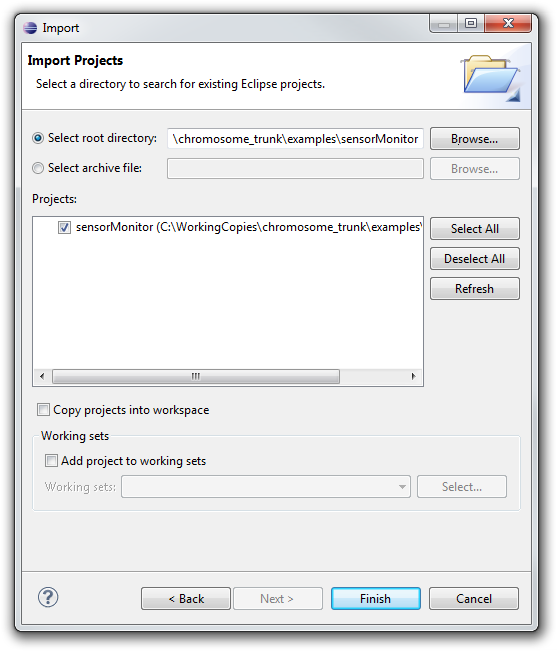
\includegraphics[scale=0.5]{figures/xme_import_sensorMonitor.png}
	\caption{Importing the \emph{sensorMonitor} project into XMT.}
	\label{fig:xmt_import_sensorMonitor}
\end{figure}

\begin{figure}[htpb]
	\centering
	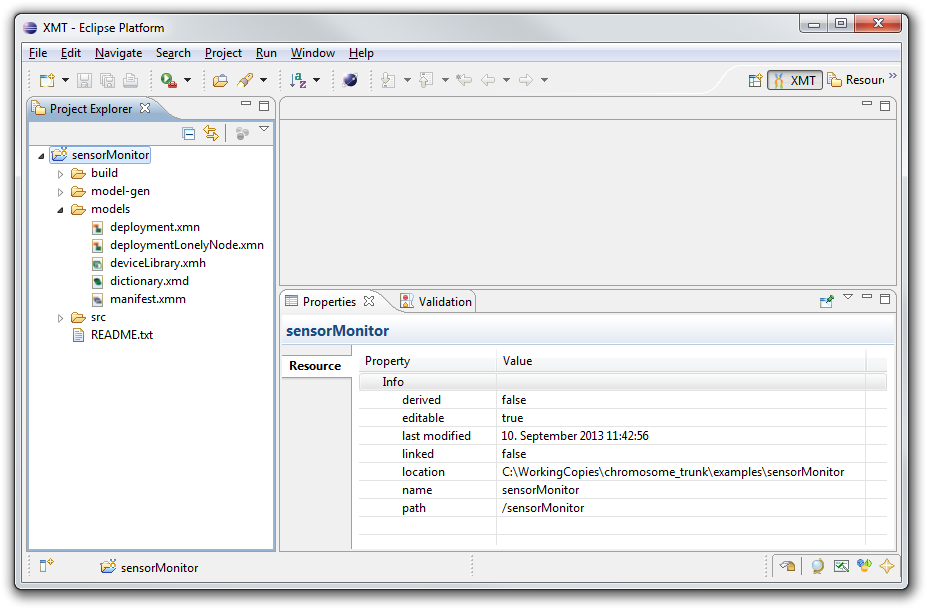
\includegraphics[width=0.9\textwidth]{figures/xmt_project_sensorMonitor.png}
	\caption{XMT perspective of \xme Modeling Tool with imported example project.}
	\label{fig:xmt_project_sensorMonitor}
\end{figure}

You already know the \verb|src/| subdirectory of this example from the previous chapter.
Now we will have a closer look at the \verb|models/| directory, which contains the XMT models that describe this application.
You can see a screenshot of the imported project with expanded models directory in Figure~\ref{fig:xmt_project_sensorMonitor}.
The directory contains five models. 
In the \emph{models} folder we can distinguish four different file extensions:

\begin{itemize}
	\item \emph{xmd} This extension stands for \emph{XMT} topic dictionary, and determines the set of topics and associated attributes to be used for the deployment of components. 
	\item \emph{xmm} This extension stands for \emph{XMT} manifest, and defines components and their interfaces. 
	\item \emph{xmh} This extension stands for \emph{XMT} device types, and is related with hardware-associated properties. 
	\item \emph{xmn} This extension stands for \emph{XMT} deployment model, and defines the mapping of components on devices and the network structure. 
\end{itemize}

In the following subsections we will have a look at these four model types, providing a short description of their purpose and demonstrating how to generate code from them.
As a preparation, we create a backup of the \verb|src/| directory in the project.
Name it something like \verb|src_backup/|. Then delete the original.
We will recreate the content step by step.
Most of the files will be generated completely by the tool.

% ~~~~~~~~~~~~~~~~~~~~~~~~~~~~~~~~~~~~~~~~~~~~~~~~~~~~~~~~~~~~~~~~~~
\subsection{Topic Dictionary}
% ~~~~~~~~~~~~~~~~~~~~~~~~~~~~~~~~~~~~~~~~~~~~~~~~~~~~~~~~~~~~~~~~~~

We begin with the \emph{topic dictionary} model.
A \emph{topic dictionary} is the collection of all topics of an application respectively application domain.
It also holds the \emph{attribute} definitions.
Attributes are attached to topics and specify additional information about the contained data.
%For example the accuracy of a measured value could be defined as an attribute.
%Additionally components can filter for certain attribute values.
%This will be explained in more detail in the chapter about the manifest model.
%\begin{itemize}
% TODO: Move this to manifest, as there are no attribute value definitions in topic dictionaries
%	\item \textbf{Attribute value definition}: The attribute definition explicitly defines pairs of \emph{\textless key, value \textgreater} associated to a topic. 
%        Attribute definitions are associated to publishers in \xme. 
%        Examples of attribute definition could be \emph{data reliability}, \emph{publication rate}, \emph{data measurement unit} or
%        \emph{time to live}. 
%  \item \textbf{Attribute filter}: The attribute filter is associated to subscribers in \xme. A filter defines a set of \emph{\textless key, value, operator\textgreater}
%	      triples, in which the operator is the comparator (\emph{EQUAL, UNEQUAL, GREATER, GREATER\_OR\_EQUAL, SMALLER, SMALLER\_OR\_EQUAL, EXISTS and NOT\_EXISTS})
%				and the value is the value to compare to the attribute definition. 
%\end{itemize}

%Additionally, we can categorize attributes as follows:
% TODO: Mandatory is wrong here, this is called required. Also I do not like this categorization and we might change it in the future...
%
%\begin{itemize}
%	\item \emph{Predefined}: Predefined attributes are specified at design time and associated attribute values do not change during the lifecycle of the application. 
%	\item \emph{Mandatory}: Mandatory attributes define the attributes that should be present in the topic at runtime and they should be provided by the application. 
%	\item \emph{Optional}: Optional attributes are those attributes that can be provided at runtime. These attributes are not mandatory, so they can be provided or not for every topic. 
%\end{itemize}
%
We will check how attributes work in the Plug and Play example (see Section~\ref{sec:example_pnp}). 

\begin{figure}[htpb]
	\centering
	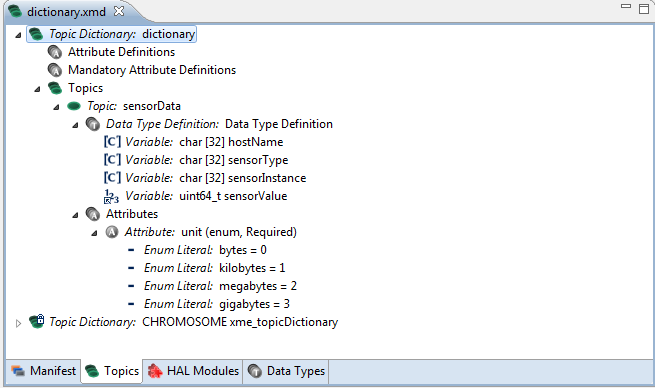
\includegraphics[scale=0.5]{figures/xmt_topicDictionary.png}
	\caption{Topic dictionary model.}
	\label{fig:xmt_topicDictionary.png}
\end{figure}

To open the model, double-click on the file \verb|models/dictionary.xmd| in the project explorer.
An editor window will open that displays the model content in a tree structure~--~see Figure~\ref{fig:xmt_topicDictionary.png}.
Additionally, the \xme \textit{xme\_topicDictionary} shows internal topics used to \xme core components like the \textit{Plug and Play Manager} and \textit{Plug and Play Client}.

You can expand items to see their sub-items.
For example, the item \emph{Topic Dictionary: dictionary} contains an item \emph{Topics} under which you can find the topic definitions.
Remember that a topic defines a type of data that can be sent between components in a \xme network (compare Section~\ref{sec:architecture:glossary}).
Topics can consist of primitive C data types or complex data structures. Additionally, we can define for each topic the set of attributes that apply to that topic. 

A double-click on an item brings the \emph{Properties} view to the foreground.
Here you can see the properties of the selected model item.
Properties may be structured in sub-properties.
When this is he case you can again expand the entry by clicking on the small triangle on the left side.
Figure~\ref{fig:xmt_sub-properties.png} shows an example for the \emph{hostName} variable of the \emph{sensorData} topic.

\begin{figure}[htpb]
	\centering
	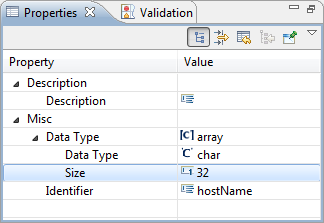
\includegraphics[scale=0.75]{figures/xmt_sub-properties.png}
	\caption{Sub-properties of a data type in the topic dictionary model.}
	\label{fig:xmt_sub-properties.png}
\end{figure}

Now let us have a closer look at the single topic defined in the example, which is called \emph{SensorData}.
In its properties, you can see a description and its name.
You can also see the ID (short for \emph{identifier}) that is used at runtime to identify this topic and its C identifier that will be used in the generated code.\footnote{%
	The identifier is automatically derived from the name of the topic and the name of the dictionary and therefore located in the property category \emph{Read-Only}.
}
Now expand every entry under the topic.
You will see that it has data type definition with several variables.
In the generated code, this will be mapped to a C struct definition.

The SensorData topic also has one attribute called ``\emph{unit}'' which is an enumeration.
It describes the measurement unit of the contained sensor value.
As in our example we measure the free hard disk size,
possible values for this attribute range from \emph{bytes} to \emph{gigabytes}.

\begin{figure}[htpb]
	\begin{minipage}[b]{0.45\linewidth}
		\centering
		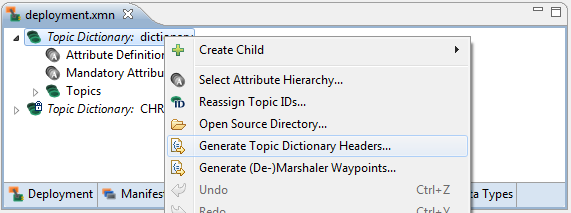
\includegraphics[scale=0.5]{figures/xmt_topicDictionary_gen_headers_a.png}
		\caption{Start topic header generation.}
		\label{fig:xmt_topicDictionary_gen_headers_a}
	\end{minipage}
	\hspace{0.5cm}
	\begin{minipage}[b]{0.45\linewidth}
		\centering
		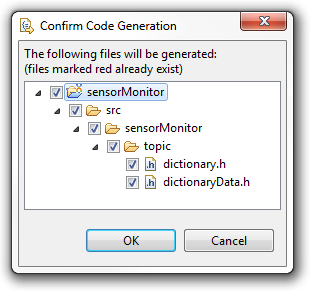
\includegraphics[scale=0.5]{figures/xmt_topicDictionary_gen_headers_b.png}
		\caption{Code generation dialog for topic headers.}
		\label{fig:xmt_topicDictionary_gen_headers_b}
	\end{minipage}
\end{figure}

For a topic dictionary two code generation commands exist.
The first option is to generate the topic headers.
To do this, right-click on the \emph{Topic Dictionary} root element and select \emph{Generate Topic Dictionary Headers...} as shown in Figure~\ref{fig:xmt_topicDictionary_gen_headers_a}.
A dialog will pop up that shows the files that will be generated~--~see Figure~\ref{fig:xmt_topicDictionary_gen_headers_b}.
You can exclude individual files by unchecking them.
Here you can see that this command will generate two files: \texttt{dictionary.h} and \texttt{dictionaryData.h}.
These contain the headers topic identifier and data type definitions that you already know from before.
Select \emph{Overwrite} and press \emph{OK} to generate the files.
After a short moment the Eclipse status line should say \emph{Code generation complete}.
You can navigate to the generated files and have a look at them if you are interested.
If the files are missing in the Eclipse \emph{Project Explorer} pane, try to refresh the \verb|src/| directory
(i.e., right-click and select \emph{Refresh} from the popup menu or select the directory item and press \emph{F5}).

The second generation command \emph{Generate (De-)marshaler waypoints...} creates marshaling and demarshaling functions for the topics of the application.
Different \xme nodes might reside on different target platforms that interpret data differently.
In order to allow these platforms to communicate with each other, the sent data must be converted into a platform independent format.\footnote{%
	For more information, see also \url{http://en.wikipedia.org/wiki/Endianness}.
}
%
The serialization of sent data to this format (i.e., from platform dependent representation to network representation)
is performed by the marshaler; the deserialization respectively by the demarshaler.
The serialization algorithm depends on the sent data~--~and so in our case on the topic definition.
To solve this issue, \xme uses a code generation approach and generates a (de-)marshaler that is specific to a dictionary.
You can start the generation by right-clicking on the \emph{Topic Dictionary} item and select \emph{Generate (De-)Marshaler Waypoints...}.
From the generated files the most interesting ones are the \verb|marshaler.c/h| and \verb|demarshaler.c/h| files, which contain the actual (de-)serialization code.

% ~~~~~~~~~~~~~~~~~~~~~~~~~~~~~~~~~~~~~~~~~~~~~~~~~~~~~~~~~~~~~~~~~~
\subsection{Manifest}
% ~~~~~~~~~~~~~~~~~~~~~~~~~~~~~~~~~~~~~~~~~~~~~~~~~~~~~~~~~~~~~~~~~~

The next model is the so called \emph{manifest}.
A manifest can be considered as a set of component blueprints.
For each component the published and subscribed topics and its functions are defined.
You can create instances of these components later in the \emph{deployment} model.

In order to open the manifest model for the \emph{sensorMonitor} example, double-click on the file \verb|models/manifest.xmm| in the \emph{Project Explorer}.
When you expand the model items, you can see that our manifest contains the several \emph{Sensor} and \emph{Monitor} component types~--~see Figure~\ref{fig:xmt_manifest.png}.
All sensors publish the \emph{sensorData} topic.
The only difference between the different sensor types are their attribute value definitions.
An attribute value definition on a publication sets an attribute of the published topic to a specific value.
This means that all data items produced at runtime will have the corresponding attribute set to the the defined value.
%
\begin{itemize}
	\item The \emph{sensorB} sets the value of attribute \emph{unit} to \emph{bytes}.
	\item The \emph{sensorKB} sets the same attribute to \emph{kilobytes}.
	\item The \emph{sensorMB} sets it to \emph{megabytes}.
\end{itemize}
%
Likewise, monitors subscribe the \emph{sensorData} topic and they differ by their attribute filters.
For example double-click on the filter of \emph{monitorKB}.
In the properties view~~see Figure~\ref{fig:xmt_filterAttributesProperties}~--~you can see the filter specification.
An attribute filter on a subscription specifies that the component is only interested in values where the attribute value satisfies certain criteria (e.g. is equal to a certain value).
%
\begin{itemize}
	\item The \emph{monitorB} component only accepts \emph{sensorData} topic data if the attribute \emph{unit} has its value set to \emph{bytes}.
	\item The \emph{monitorKB} does the same except that the value needs to be \emph{kilobytes}.
	\item The \emph{monitorMB} the same again for \emph{megabytes}.
\end{itemize}
%

\begin{figure}[htpb]
	\centering
	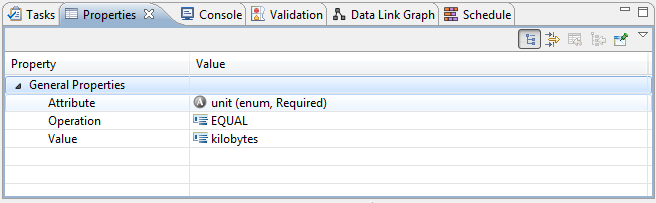
\includegraphics[scale=0.5]{figures/xmt_filterAttributesProperties.png}
	\caption{Attribute filter properties window.}
	\label{fig:xmt_filterAttributesProperties}
\end{figure}

Additionally, there is a manifest called \xme \emph{xme\_manifest} which contains \emph{core} components. 
The code for these components is located in the \verb|<XME_ROOT>/xme/core| directory.
We will not need the core components in this section.

\begin{figure}[htpb]
	\centering
	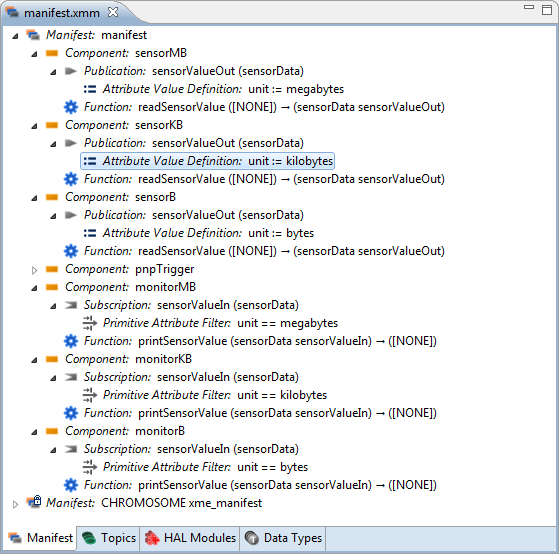
\includegraphics[scale=0.6]{figures/xmt_manifest.png}
	\caption{Manifest model.}
	\label{fig:xmt_manifest.png}
\end{figure}

From the manifest model you can initiate the generation of the so called component and function wrappers and a stub for the function implementation.
Right-click on the \emph{Manifest: sensorMonitor} item and select \emph{Generate Component Wrappers...}.
In the emerging dialog you can see a list of the generated files.

Wrappers constitute the necessary glue code between the function's implementation and the middleware (see also Section~\ref{sec:architecture:glossary}).
These are generated completely from the model and do not need to be adapted.
The files \verb|printSensorValueFunction.c| and \verb|readSensorValueFunction.c| are where the actual functionality of the components are implemented.
Press \emph{OK} to generate all files and open both source files from the \emph{sensorB}.
The generated implementation simply does nothing in its \emph{init()}, \emph{step()} and \emph{fini()} functions.
%
Consider the following excerpt:
%
\begin{lstlisting}[breaklines]
void
sensorMonitor_adv_sensorB_readSensorValueFunction_step
(
	void* param
)
{
    xme_status_t status[1];
    
    sensorMonitor_topic_sensorData_t* portSensorValueOutDataPtr =
        &portSensorValueOutData;
    
    {
        // PROTECTED REGION ID(SENSORMONITOR_ADV_SENSORB_READSENSORVALUEFUNCTION_STEP_C) ENABLED START
\end{lstlisting}
\vspace{-\baselineskip}
\begin{lstlisting}[breaklines, backgroundcolor=\color{yellow}, escapechar=\%]
%%
	// TODO: Auto-generated stub

	XME_UNUSED_PARAMETER(param);
        XME_UNUSED_PARAMETER(status);
%%
\end{lstlisting}
\vspace{-\baselineskip}
\begin{lstlisting}[breaklines]
	// PROTECTED REGION END
    }
	
    status[0] = sensorMonitor_adv_sensorB_sensorBComponentWrapper_writePortSensorValueOut(portSensorValueOutDataPtr);
    
    {
        // PROTECTED REGION ID(SENSORMONITOR_ADV_SENSORB_READSENSORVALUEFUNCTION_STEP_2_C) ENABLED START
\end{lstlisting}
\vspace{-\baselineskip}
\begin{lstlisting}[breaklines, backgroundcolor=\color{yellow}, escapechar=\%]
    
        // TODO: Auto-generated stub
        //       Check return values of writePort calls here
    %%
\end{lstlisting}
\vspace{-\baselineskip}
\begin{lstlisting}[breaklines]
        // PROTECTED REGION END
    }
}
\end{lstlisting}

The \lstinline|// TODO: Auto-generated stub| comments mark where you can add your own implementation of the respective function.
%
In this example, these files are the only thing that you need to manually adjust to recreate the example from the previous chapter.
Just copy these files over from your backup and replace the generated versions.
The code listing above shows the generated \verb|step()| function for the sensor component.

Notice the comments which are marked with \lstinline|// PROTECTED REGION|.
These regions enclose a section of code~--~marked yellow in the code listing~--~that will not be modified by the tool when regenerating the code.
You can verify this by starting the code generation again. Do not modify or remove the protected region comments.
This time before pressing \emph{OK}, have a look at the \emph{Select Merge Strategy} section.
Figure~\ref{fig:xmt_manifest_protected_regions.png} shows the bottom of the code generation dialog with the protected regions strategy highlighted.
This section tells the tool what to do when a generated file already exists.\footnote{%
	Existing files are marked red in the dialog.
}
\begin{enumerate}
	\item The \emph{Compare Editor} option will open a compare editor for every differing file.
		There you can manually select which parts to use from the generated code and which part to keep.

	\item The second option \emph{Protected Regions} will preserve any code in the protected regions.
		Select this option and press \emph{OK}.
	
	\item The third option \emph{Overwrite} will simply overwrite existing files with generated content~--~use with caution.
\end{enumerate}
%
Choose Protected Regions and verify that the content in the protected regions is kept intact.

\begin{figure}[htpb]
	\centering
	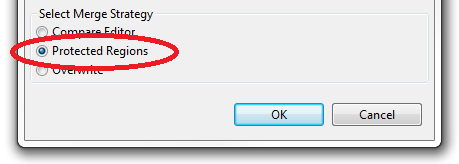
\includegraphics[scale=0.50]{figures/xmt_manifest_protected_regions.png}
	\caption{Code generation dialog with protected region merge strategy selected.}
	\label{fig:xmt_manifest_protected_regions.png}
\end{figure}

% ~~~~~~~~~~~~~~~~~~~~~~~~~~~~~~~~~~~~~~~~~~~~~~~~~~~~~~~~~~~~~~~~~~
\subsection{Device Types}
% ~~~~~~~~~~~~~~~~~~~~~~~~~~~~~~~~~~~~~~~~~~~~~~~~~~~~~~~~~~~~~~~~~~

The \emph{device types} model is a very simple description of hardware devices on which your \xme executables run.
A device type has a \emph{Target Identifier} which specifies the platform (e.g., \emph{posix}, \emph{windows}\footnote{%
	Currently these are the only officially supported platforms.
}).
A device type also has several network interfaces. Currently only \emph{ethernet} is supported.
You will be able to create instances of these devices in the deployment model.

To open the model, double-click on the file \verb|models/deviceTypes.xmn| in the project explorer~--~see Figure~\ref{fig:xmt_deviceTypes.png}.
It contains only a simple device with a single Ethernet interface.
The \emph{target identifier} is deliberately left empty.
In this case, the \xme build system will automatically detect the build environment and assume it to be the execution environment.

\begin{figure}[htpb]
	\centering
	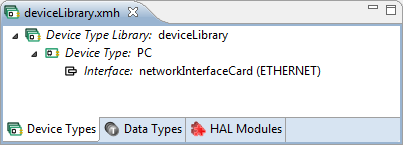
\includegraphics[scale=0.75]{figures/xmt_deviceTypes.png}
	\caption{Device types model.}
	\label{fig:xmt_deviceTypes.png}
\end{figure}

% ~~~~~~~~~~~~~~~~~~~~~~~~~~~~~~~~~~~~~~~~~~~~~~~~~~~~~~~~~~~~~~~~~~
\subsection{Deployment}
% ~~~~~~~~~~~~~~~~~~~~~~~~~~~~~~~~~~~~~~~~~~~~~~~~~~~~~~~~~~~~~~~~~~

The \emph{deployment} model ties everything together.
Here you specify devices and nodes and specify which components are deployed on which node.
In the future you will also be able to specify the network structure here,
which will allow the tool to calculate routes for your network and configure your nodes accordingly.\footnote{%
	Actually you can already define the network structure, but this information is currently not used.
}

To open the model, double-click on the file \verb|models/deployment.xmn| in the project explorer~--~see Figure~\ref{fig:xmt_deployment.png}.
This example contains three nodes.
The \emph{monitorNode} contains the monitor component and the \emph{monitorNode} contains the sensor component.
There are also other components and an additional node that you will get to know in the next chapters.

\begin{figure}[htpb]
	\centering
	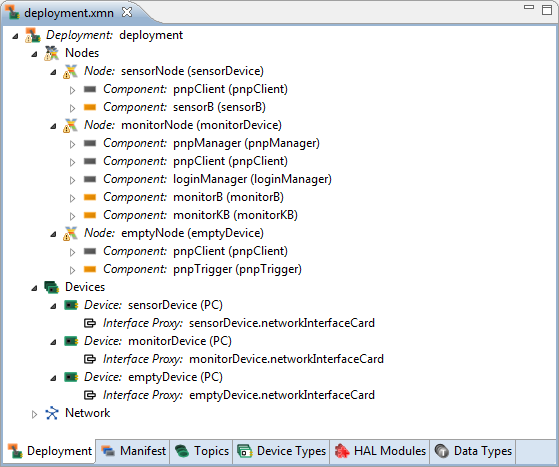
\includegraphics[scale=0.75]{figures/xmt_deployment.png}
	\caption{Fully expanded deployment model.}
	\label{fig:xmt_deployment.png}
\end{figure}

A node here refers to a \xme executable.
Components from the manifests can be instantiated on each node.
You can also instantiate the same component multiple times on the same node (though the example does not include such a case).

A device represents a hardware device on which one or several nodes can be run.
Usually you run only one \xme executable per device, but there might be exceptions.
A device is an instantiation of a type defined in a device types model.
This allows to reuse a device definition.
In addition to the information from the type, you have to specify a network address for each interface.

In the deployment model you can generate the main source file for a node, which will start a \xme instance.
This main source file will also set up the \xme configuration as determined by the tool.
Additionally the CMake scripts are generated that allow you to build your application.
To start the code generation, right-click on the \emph{Deployment: deployment} item and select \emph{Generate Application Code...}
(compare Figure~\ref{fig:xmt_deployment_generate}).
%
\begin{figure}[ht]
	\centering
	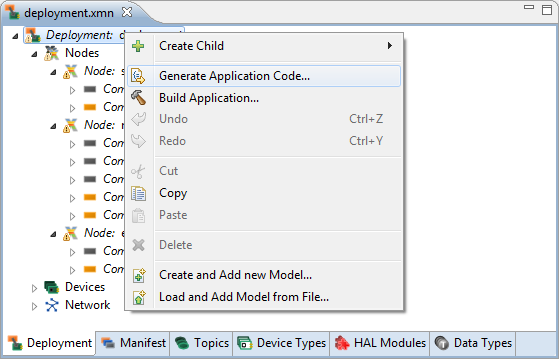
\includegraphics[scale=0.55]{figures/xmt_deployment_generate.png}
	\caption{Generation of application code from a deployment model.}
	\label{fig:xmt_deployment_generate}
\end{figure}
%
There will be three files per node.
The \verb|sensorNode.c| respectively \verb|monitorNode.c| are the aforementioned main source files.
The \verb|CMakeLists.txt| is the main CMake script for the respective node.
The file \verb|CMakeXmeComponents.txt| is included by the main CMake script and contains a definition of all components on that node, so that the build system is aware of them.

When clicking on \emph{Generate Application Code...} you can also see that two new views, called \emph{Data Link Graph} and \emph{Schedule}, pop up.
First let us have a look at the data link graph view.
Screenshot~\ref{fig:xmt_dataLinkGraphView} shows a cutout from this view.
The data link graph is a representation of the resulting data paths in the application.
Beginning from publications and ending at subscriptions it shows the path along which data is sent.
First the XMT searches for matching publications and subscriptions (where the topics are equal and attribute filters match).
For each match a so called logical route is added.
Afterwards these logical routes are refined by adding waypoints.
For example you can have a look at the data path from the publication \verb|sensorB.sensorValueOut| to the subscription \verb|monitorB.sensorValueIn|.
As they lie on different nodes, the data has to be sent across the network.
For this purpose four waypoints have been added, namely: Marshaler, UdpSend, UdpReceive, and Demarshaler.
Data sent from the publication first goes to the Marshaler which serializes the data into a platform independent format.
Next it will be processed by the UdpSend waypoint which sends the data across the network via UDP to the correct receiver(s).
On the receiving node, the UdpReceive waypoint receives the data and passes it to the Demarshaler who deserializes the data again before giving it to the subscription,
where it will be read by the application.

\begin{figure}[ht]
	\centering
	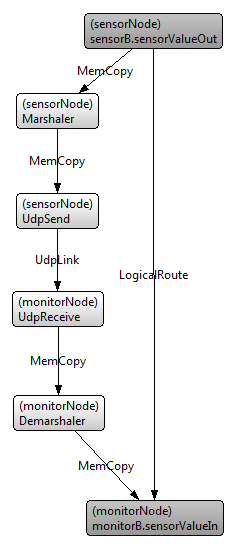
\includegraphics[scale=0.75]{figures/xmt_dataLinkGraphView.png}
	\caption{Cutout from Data Link Graph View.}
	\label{fig:xmt_dataLinkGraphView}
\end{figure}

The other new view is the schedule view.
Here you can see a visualization of the schedule for each node in the deployment model.
For this example it will look like shown in screenshot~\ref{fig:xmt_scheduleView}.
Each node is displayed on a separate line and each line represents one schedule cycle.
Next to the name of a node are colored boxes for each schedule entry.
The purple ones correspond to waypoints, the orange one to functions from components.
The numbers in the boxes are the slot length in milliseconds
and in brackets the number n, where n means that this will be executed only every n-th cycle of the schedule.
The length of a box is proportional to the slot length.
You can hover the mouse cursor over a schedule entry to see a tool tip with more detailed information.

\begin{figure}[ht]
	\centering
	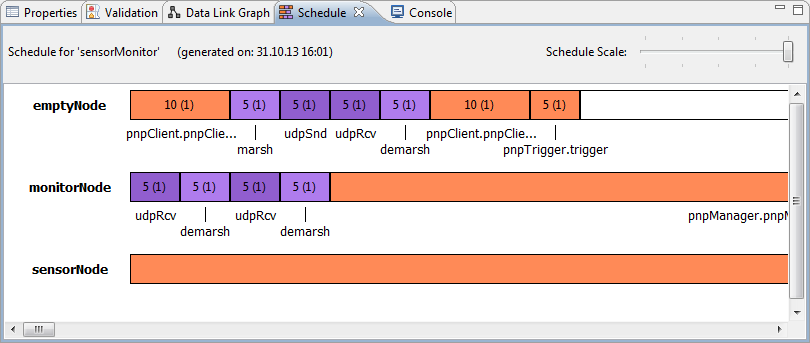
\includegraphics[scale=0.75]{figures/xmt_scheduleView.png}
	\caption{Schedule View.}
	\label{fig:xmt_scheduleView}
\end{figure}

You may now compile the generated code as presented in the previous section or directly use \xmt to build the code as follows:
right-click on the \emph{Deployment: deployment} node in the model
and select \emph{Build Application...}~--~see Figure~\ref{fig:xmt_deployment_generate}.

After clicking on this context menu option, a new window will appear.
This window allows to set up the nodes that are going to be compiled.
The required CMake build system will be automatically created in this case.
%
Note that the nodes that appear in this window are directly related to the deployment model (compare Figure~\ref{fig:xmt_deployment_buildWindow}).
The first option (\emph{Generate Build System}) will generate all the files needed for building the system\footnote{%
	Currently, the build system is associated to a build in Visual Studio.
	In case you want to use a different compiler toolchain, you have to manually adapt the generated \texttt{CMakeLists.txt} file.
}.
The second option is related to with compilation of the generated build.

\begin{figure}[ht]
	\centering
	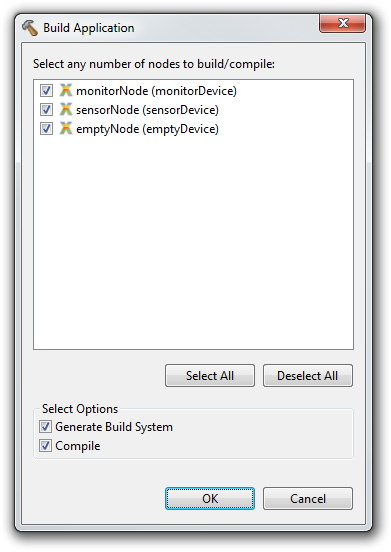
\includegraphics[scale=0.75]{figures/xmt_deployment_buildWindow.png}
	\caption{XMT build options.}
	\label{fig:xmt_deployment_buildWindow}
\end{figure}

% ~~~~~~~~~~~~~~~~~~~~~~~~~~~~~~~~~~~~~~~~~~~~~~~~~~~~~~~~~~~~~~~~~~
\subsection{Conclusion}
\label{sec:example_xmt:conclusion}
% ~~~~~~~~~~~~~~~~~~~~~~~~~~~~~~~~~~~~~~~~~~~~~~~~~~~~~~~~~~~~~~~~~~

If you followed all previous steps, you have generated the complete application and should be able to compile and run it again like described in Section~\ref{sec:example_sensorMonitor}.

Alternatively you can use also trigger compilation from inside the XMT.
For this you first have to enter some CMake related settings.
Go to \textit{Window $\rightarrow$ Preferences}.
In the preferences dialog expand the \textit{XMT} item and click on the sub-item \textit{CMake}.
Set the path to the CMake executable by pressing \emph{Browse...} and navigating to the respective file.
Then choose the correct generator from the drop-down list.
You only have to do these steps once.
Now you can trigger build system generation and compilation.
Go to the deployment model and right-click on the deployment item.
Choose \emph{Build Application...}.
Select the nodes that you want to build and check if you want to generate the build system or compile the selected nodes (or both).
When pressing \emph{OK} the tool will start CMake and print its output to the Console view.

You are now free to modify the models, re-generate the source code and change the behavior of the components.
One interesting example is to change the IP addresses of the nodes and deploy them on different machines in a local-area network.
Notice however that you might need to add respective exceptions in your firewall.
The default ports being used in this example are 33221 for \textit{monitor} node, 33222 for \textit{sensor} node and 33223 for \textit{empty} node.
More on the topic of distributed applications will come in the next release of \xme (see our roadmap in Appendix~\ref{appx:roadmap}).
